%%%%%%%%%%%%%%%%%%%%%%%%%%%%%%%%%%%%%%%%%%%%%%%%%%%%%%%%%%%%%%%%%%%%
\section{Anode Plane Assembly (APA) Overview}
\label{sec:fdsp-apa-intro}

Anode planes (or wire planes) are the DUNE \dword{spmod} elements used to sense, through both signal induction and direct collection, the ionization electrons created when charged particles traverse the \lar volume inside the \dword{spmod}. To facilitate fabrication and installation underground, the anode design is modular, with \dwords{apa} tiled together to form the readout system for a \SI{10}{kt} \dword{detmodule}. A single \dword{apa} is \SI{6}{m} high by \SI{2.3}{m} wide, but two of them are connected vertically, and twenty-five of these vertical stacks are linked together to define a \SI{12}{m} tall by \SI{58}{m} long mostly-active readout plane.  As described below, the planes are active on both sides, so three such wire readout planes are interleaved with two high voltage surfaces to define four \SI{3.6}{m} wide drift regions inside each \dword{spmod}, as shown in the detector schematic views in Figure~\ref{fig:FarDet-interior}.  Each single-phase \SI{10}{kt} module, therefore, will contain 150 \dwords{apa}.

\begin{dunefigure}[Schematic view of a DUNE \SI{10}{kt} \dword{spmod} %single phase TPC module
]{fig:FarDet-interior}
{Left: End-on schematic view of the active argon volume showing the four drift regions and anode-cathode plane ordering of the TPC inside the detector. Right: View of the partially installed DUNE TPC inside the membrane cryostat. The \dwords{apa} are shown in red, \dwords{cpa} are in cyan, \dword{fc} modules in yellow/green.  Some of the \dword{fc} modules are in their folded position against the cathode to providing aisle access during installation.}
\setlength{\fboxsep}{0pt}
\setlength{\fboxrule}{0.5pt}
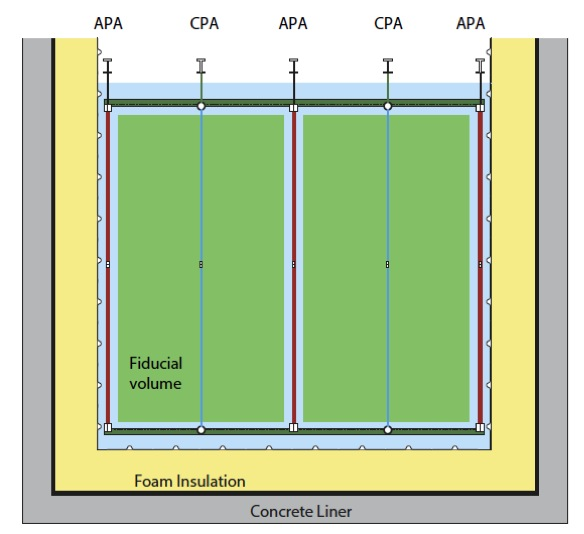
\includegraphics[width=0.445\textwidth, trim=0mm 3.7mm 0mm 0mm, clip]{apa-dune-sp-endview.jpg}\hspace{0.01\textwidth}
\fbox{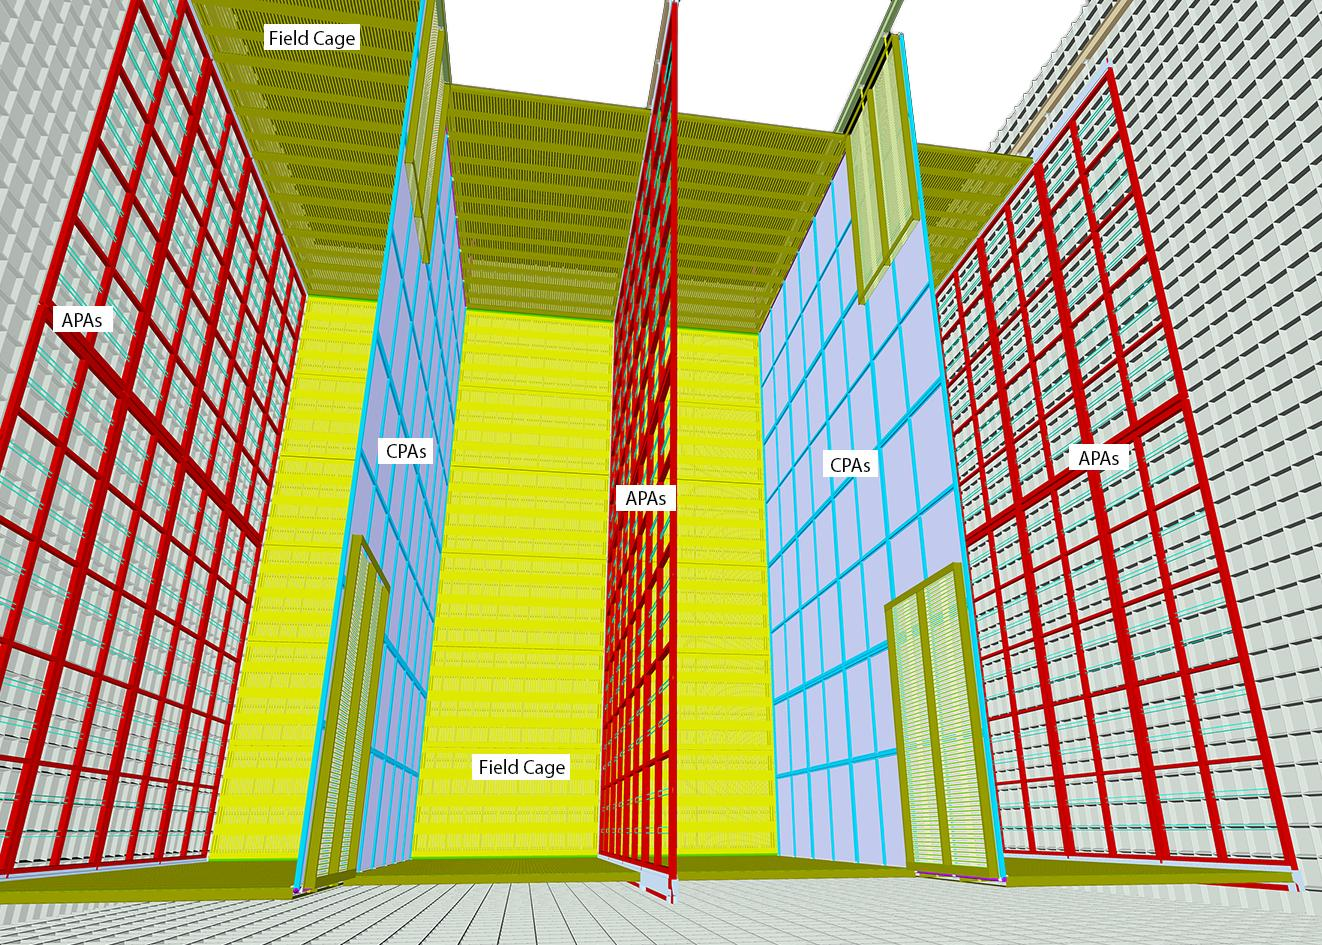
\includegraphics[width=0.52\textwidth]{apa-dune-sp-floor-view.jpg}}
\end{dunefigure}

Each \dword{apa} frame is covered by over \num{2500} sense wires laid in three planes  oriented at angles to each other: a vertical collection plane, $X$, and two induction planes at $\pm35.7^\circ$ to the vertical, $U$ and $V$. These enable multi-dimensional reconstruction of particle tracks.  An additional \num{960} wires that are not read out make up an outer shielding plane, $G$, to improve signal shapes on the $U$ induction channels.  The angled wires are wrapped around the frame from one side to the other, allowing all channels to be read out from one end of the \dword{apa} only (the top or bottom), and thereby minimizing the dead regions between neighboring \dwords{apa}. Signals induced or collected on the wires are transferred through soldered connections to wire termination boards mounted at the end of the \dword{apa} frame that in turn connect to \dword{fe} readout electronics sitting in the \lar.  Figures~\ref{fig:tpc_apa1} and \ref{fig:tpc_apa2} illustrate the layout of the wires on an \dword{apa}, showing how they wrap around the frame and terminate on wire boards at the head end where readout electronics are mounted.

The \dwords{apa} represent a critical interface point between the various detector subsystems within the \dword{spmod}.  As already mentioned, the TPC readout electronics mount directly to the \dword{apa} frames.  \Dwords{pd} for detecting scintillation light produced in the \lar are also housed inside the frames, sandwiched between the wires on the two sides, requiring careful coordination in the frame design as well as placing a requirement on the transparency of the \dword{apa} structures.  In addition, the electric \dfirst{fc} panels connect directly to the edges of the \dword{apa} frames.  Finally, the \dwords{apa} must support the routing of cables for both the TPC electronics and the photon detector systems. All of these considerations have important impacts on the design, fabrication, and installation planning for the \dwords{apa}.   

\begin{dunefigure}[Illustration of the \dword{apa} wire layout]{fig:tpc_apa1}
{Illustration of the DUNE \dword{apa} wire wrapping scheme showing small portions of the wires from the three signal planes ($U,V,X$). The fourth wire plane ($G$) above these three, and parallel to $X$, is present to improve the pulse shape on the $U$ plane signals. The TPC electronics boxes, shown in blue on the right, mount directly to the frame and process signals from both the collection and induction channels. The \dword{apa} is shown turned on its side in a horizontal orientation.} 
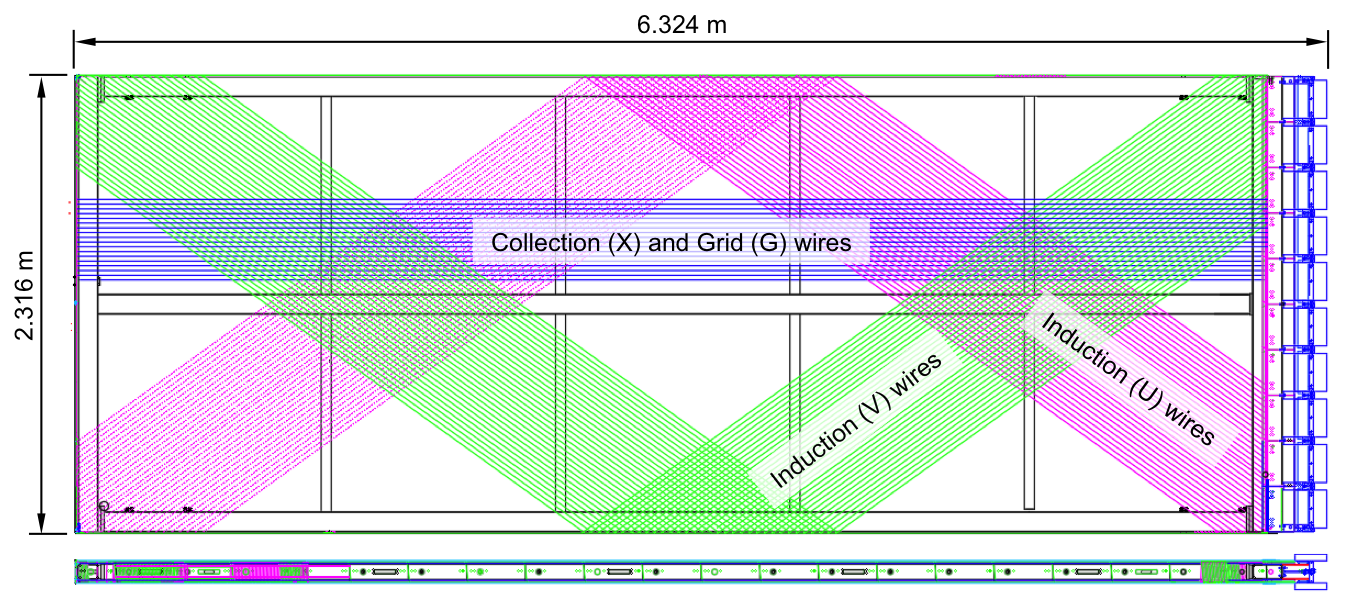
\includegraphics[width=\textwidth]{apa-drawing-wire-configuration.png} 
\end{dunefigure} 

\begin{dunefigure}[Cross section view of the head end and wire layers of an \dword{apa}]{fig:tpc_apa2}
{Cross section view of an \dword{apa} frame near the head end showing the layers of wires ($X,V,U,G$ inside to out) on both sides of the frame and terminating on wire boards at the head end of the frame, which connect directly to TPC readout electronics.} 
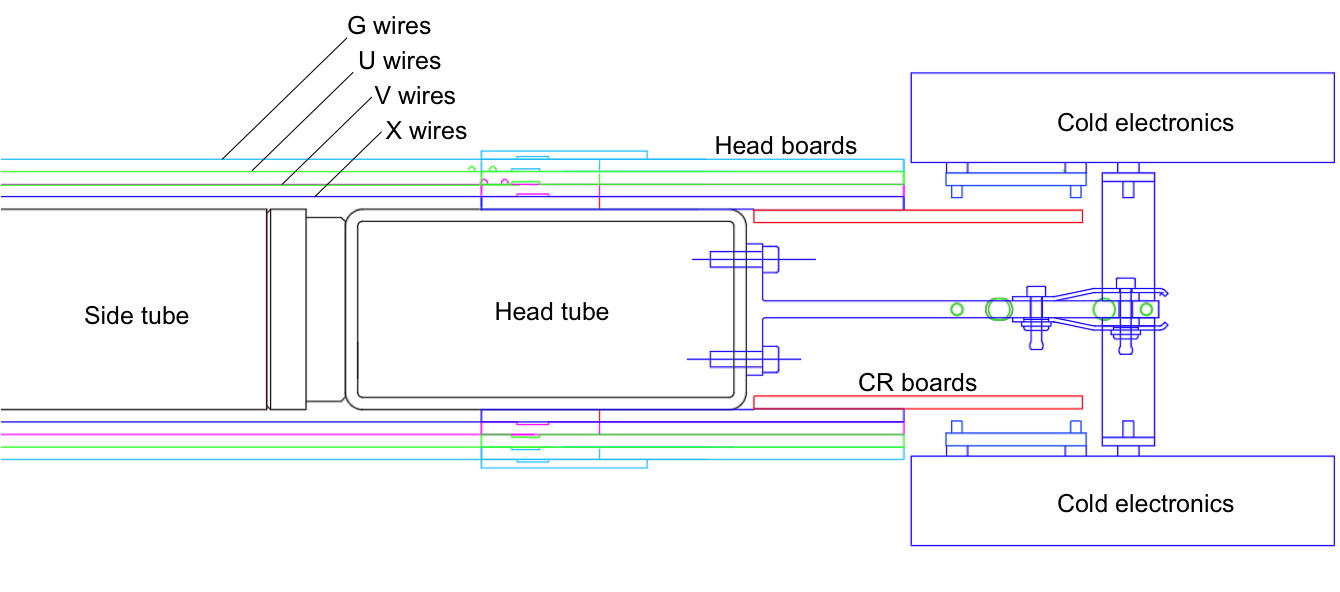
\includegraphics[width=0.95\textwidth]{apa-drawing-cross-section.png} 
\end{dunefigure} 

Full-scale \dwords{apa} have recently been produced at the Physical Sciences Laboratory (PSL) at the University of Wisconsin and at the Daresbury Laboratory in the UK for the \dword{pdsp} project at CERN. Figure~\ref{fig:apa-photo} shows a completed \dword{apa} produced at PSL just before shipment to CERN for use in \dword{pdsp}. This effort has greatly informed the design and production planning for the DUNE \dwords{detmodule}, and future \dword{pdsp} running is expected to provide valuable validation information for many fundamental aspects of the  \dword{apa} design. 

The design, construction, testing, and installation of the \dwords{apa} is overseen by the \dword{apa} consortium within the DUNE collaboration. Multiple \dword{apa} production sites will be set up in the USA and the UK, with each nation producing approximately half of the \dwords{apa} needed for the %DUNE 
\dwords{spmod}.  Factory setup is anticipated to begin in 2020, with \dword{apa} fabrication for the first \SI{10}{kt} far detector module running from 2021--2023.  

\begin{dunefigure}[Photo of a completed \dword{pdsp} \dword{apa}.]{fig:apa-photo}
{Completed \dword{pdsp} \dword{apa} ready for shipment to CERN.}
\setlength{\fboxsep}{0pt}
\setlength{\fboxrule}{0.5pt}
\fbox{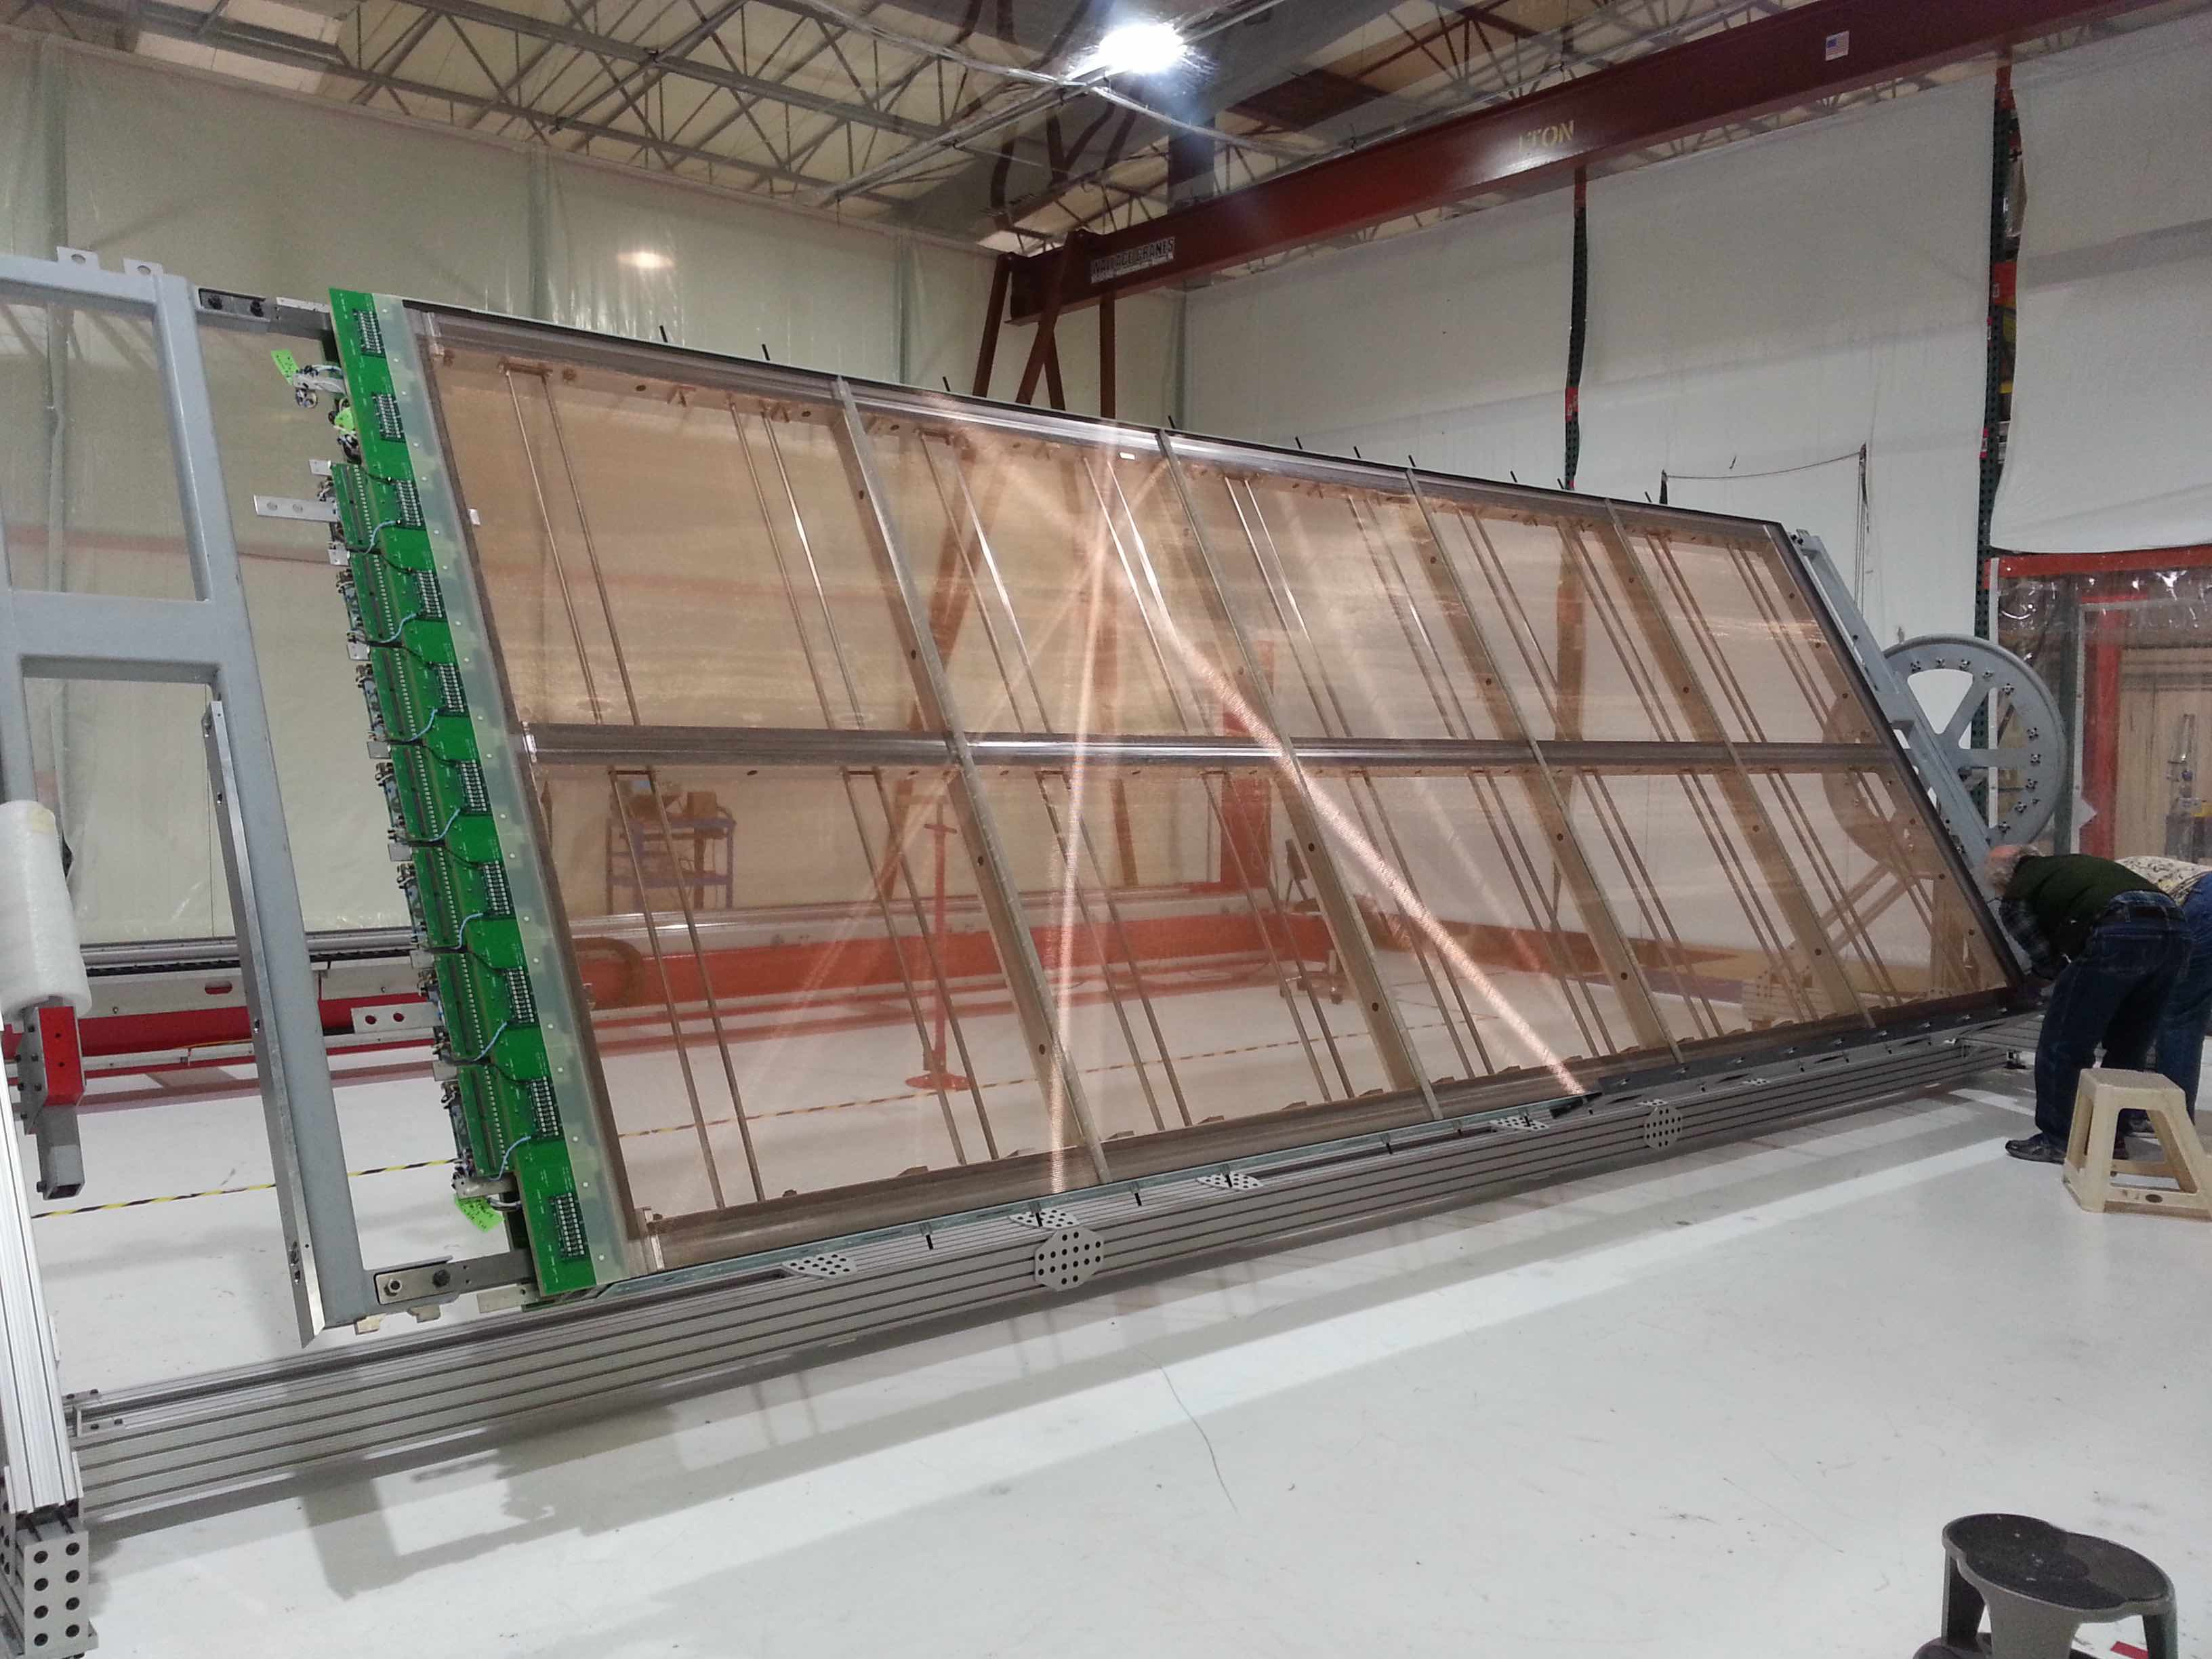
\includegraphics[width=0.9\textwidth,trim=20mm 80mm 0mm 60mm,clip]{apa-photo-complete.jpg}} 
\end{dunefigure}
